\documentclass{article}
\usepackage[utf8]{inputenc}
\usepackage{amsmath}
\usepackage{amsfonts}
\usepackage{amssymb}
\usepackage{graphicx}
\usepackage{geometry}
\usepackage{xcolor}
\usepackage{gensymb}

\newcommand{\inv}{^{-1}}   
\newcommand{\Z}{\mathbb Z}
\newcommand{\R}{\mathbb R}
\newcommand{\Q}{\mathbb Q}
\newcommand{\C}{\mathbb C}
\newcommand{\N}{\mathbb N}

\begin{document}
\pagecolor{black}
\color{white}

\noindent{\bf 1.}

    To make an $8\Omega$, $1W$ resistor, simply connect one pair of $8\Omega$, $\frac14W$ resistors in parallel, then do the same for the other pair, and then connect the two parallel components in series, as shown in the diagram below:

    \begin{center}
    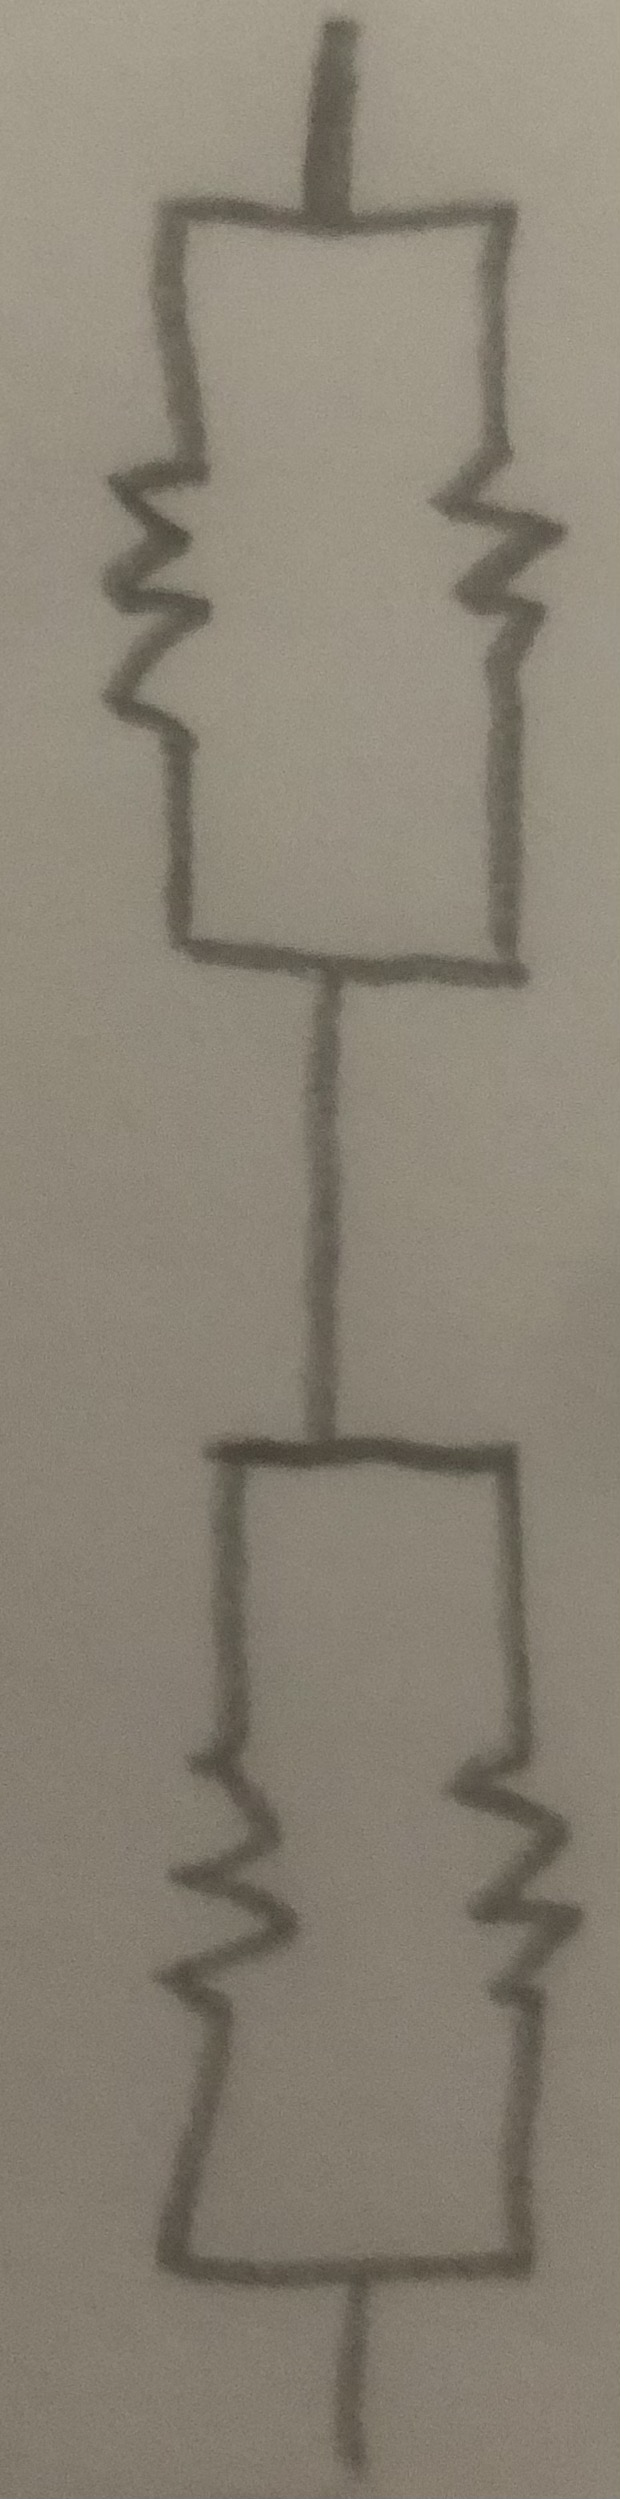
\includegraphics[angle=90,scale=.1]{resistors.jpg}
    \end{center}

\bigskip
\noindent{\bf 2.}

    \begin{center}
    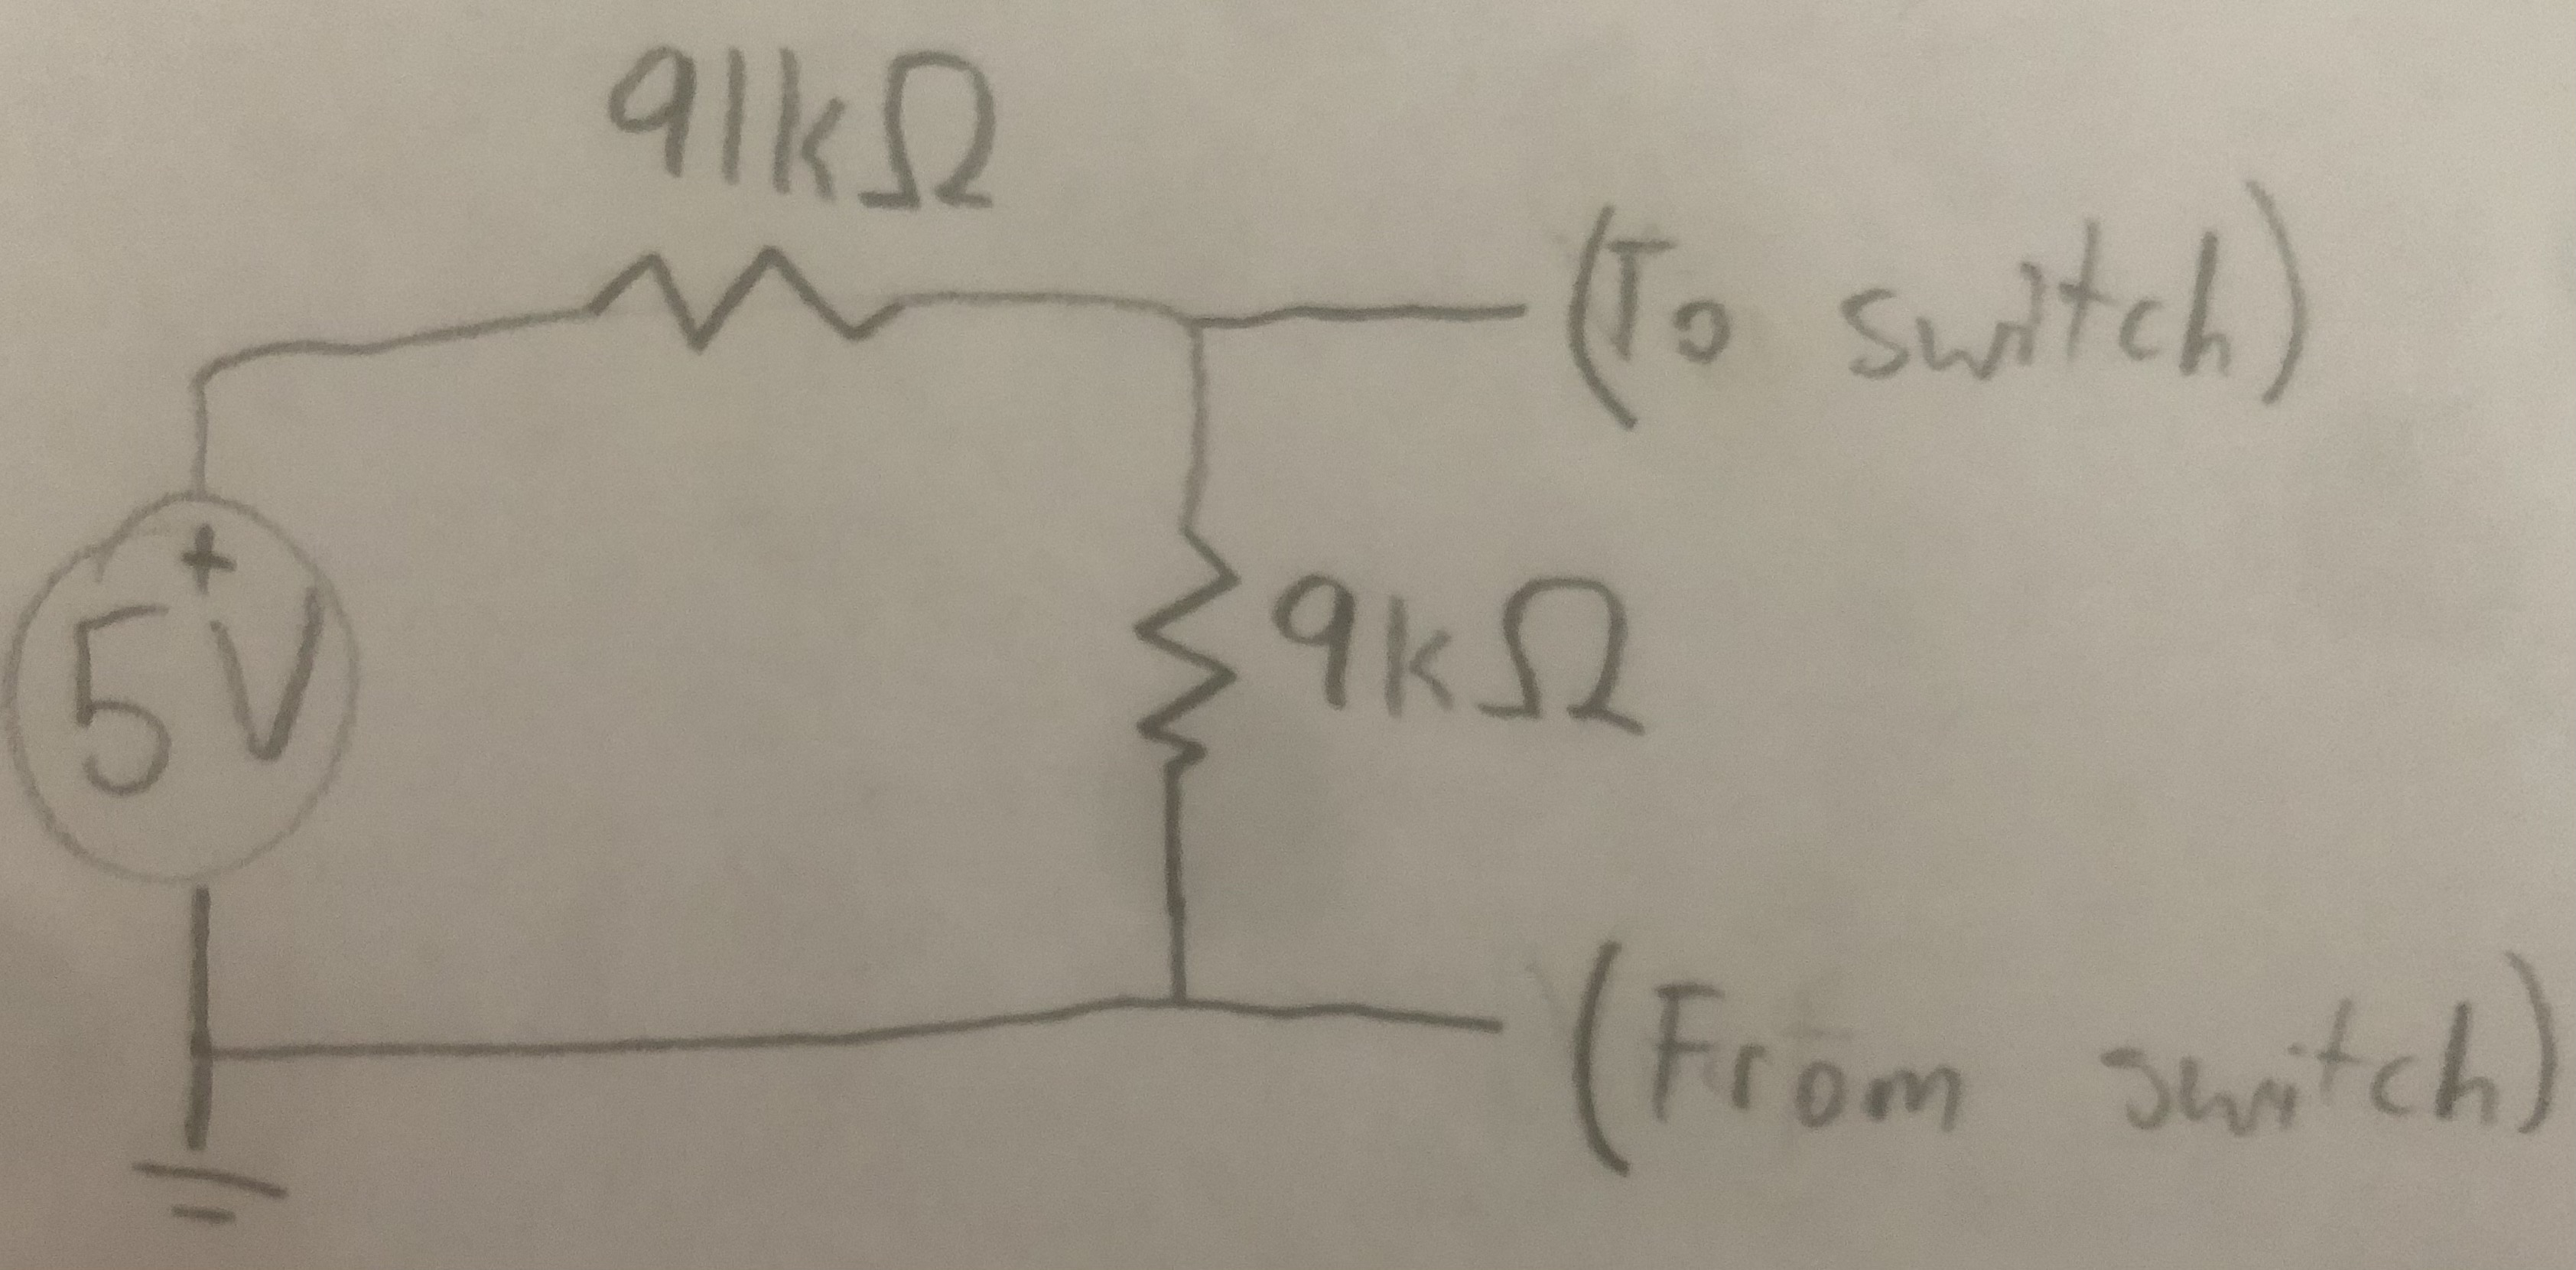
\includegraphics[scale=.1]{switch_circuit.jpg}
    \end{center}

\newpage
\noindent{\bf 3.}

{\bf (a)} $$2\cdot\frac{1.6}{10}=.32\Omega.$$

\medskip
{\bf (b)}
\begin{align*}
    P &= IV \\
    2000 &= I(115), \\
    \implies I &= \frac{400}{23}\text{A}.
\end{align*}
Thus,
\begin{align*}
    P &= I^2R \\
    2000 &= \left(\frac{400}{23}\right)^2 \cdot R, \\
    \implies R &= \frac{529}{80} \\
    &\approx 6.61\Omega.
\end{align*}

\medskip
{\bf (c)} The total resistance of the toaster plus wires is $6.93\Omega$.

\medskip
{\bf (d)}
\begin{align*}
    V &= IR \\
    115 &= I(6.93), \\
    \implies I &\approx 16.59\text{A}.
\end{align*}

\medskip
{\bf (e)}
\begin{align*}
    P_{\text{wires}} &= I^2R \\
                     &= 16.59^2 \cdot .32 \\
                     &\approx 88.07W \\
    P_{\text{toaster}} &= I^2R \\
                       &= 16.59^2 \cdot 6.61 \\
                       &\approx 1819W
\end{align*}

\newpage
\noindent{\bf 3. (Again?)}

In the diagram below, let all currents flow right through horizontal resistors, and down through vertical resistors.
Let the voltages at the red, blue, green and yellow nodes be denoted $V_R$, $V_B$, $V_G$, and $V_Y$, respectively.
\begin{center}
    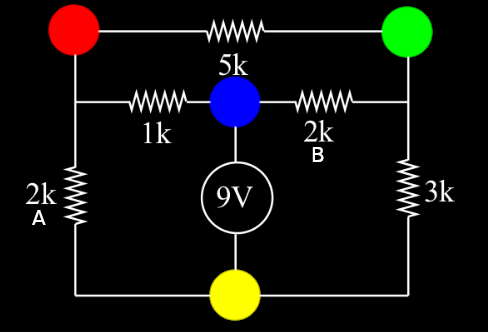
\includegraphics[scale=.65]{circuit.png}
\end{center}
Thus, $V_B = 9$, and $V_Y = 0$.
Then, $$I_{3k} = \frac{V_G - V_Y}{3000},~~~ I_{5k} = \frac{V_R - V_G}{5000},~~~ I_{1k} = \frac{V_R - V_B}{1000},~~~ I_{2k(A)} = \frac{V_R - V_Y}{2000},~~~ I_{2k(B)} = \frac{V_B - V_G}{2000},$$
and $$I_{5k} + I_{2k(B)} = I_{3k},~~~ 0 = I_{1k} + I_{2k(A)} + I_{5k}.$$
Thus,
\begin{align*}
             0   &= I_{1k} + I_{2k(A)} + I_{5k} \\
                 &= \frac{V_R - V_B}{1000} + \frac{V_R - V_Y}{2000} + \frac{V_R - V_G}{5000} \\
                 &= \frac{V_R - 9}{1000} + \frac{V_R}{2000} + \frac{V_R - V_G}{5000}, \\
    \implies V_G &= \frac{17}2V_R - 45.
\end{align*}
Then,
\begin{align*}
    I_{3k}                 &= I_{5k} + I_{2k(B)} \\
    \frac{V_G - V_Y}{3000} &= \frac{V_R - V_G}{5000} + \frac{V_B - V_G}{2000} \\
    \frac{V_G}{3000}       &= \frac{V_R - V_G}{5000} + \frac{9 - V_G}{2000}, \\
    \implies V_G           &= \frac{6}{31}V_R+\frac{135}{31}.
\end{align*}
Thus,
\begin{align*}
    \frac{17}2V_R - 45 &= \frac{6}{31}V_R+\frac{135}{31}, \\
    \implies V_R       &= \frac{\left(\frac{135\cdot62}{31}+45\cdot62\right)}{17\cdot31-12} \\
                       &\approx 5.94V.
\end{align*}
Therefore,
\begin{align*}
    V_G &= \frac{17}2\frac{\left(\frac{135\cdot62}{31}+45\cdot62\right)}{17\cdot31-12} - 45 \\
        &\approx 5.50V.
\end{align*}
Finally,
\begin{align*}
    I_{3k}    &= \frac{V_G - V_Y}{3000} \approx 1.83mA \\
    I_{5k}    &= \frac{V_R - V_G}{5000} \approx 87.38\mu A \\
    I_{1k}    &= \frac{V_R - V_B}{1000} \approx -3.06mA \\
    I_{2k(A)} &= \frac{V_R - V_Y}{2000} \approx 2.97mA \\
    I_{2k(B)} &= \frac{V_B - V_G}{2000} \approx 1.75mA
\end{align*}

\noindent\newpage{\bf 4.}
\begin{align*}
    V &= IR, \\
    \implies 1 &= I \cdot 1000, \\
    \implies I &= \frac1{1000}\Omega.
\end{align*}
Thus, the peak power dissipated in the resistor is $$I^2R = \left(\frac1{1000}\right)^2 \cdot 1000 = \frac{1}{1000}\text{W}.$$

The RMS voltage of the AC source is $\frac1{\sqrt{2}}$V, so the average power dissipated in the resistor is $\frac{\left(\frac1{\sqrt2}\right)^2}{1000} = \frac1{2000}$W.

\noindent\newpage{\bf 5.}

    Since we have the RMS voltage, we can solve for the resistance of the stove:
    \begin{align*}
             P              &= IV, \\
    \implies 1200           &= I \cdot 230 \\
    \implies \frac{120}{23} &= I
    \end{align*}
    \begin{align*}
             V &= IR, \\
    \implies 230 &= \frac{120}{23} \cdot R, \\
    \implies R &= \frac{23 \cdot 23}{12} \\
               &= 529\Omega.
    \end{align*}
    Thus, the resistance of the stove element is $529\Omega$.

    Since the RMS voltage of the AC power supply is 230V, its peak-to-peak voltage is about 650V.

\noindent\bigskip{\bf 6.}

The amplitude of the solid wave is 0.7V.

The RMS voltage of the solid wave is $\frac{1}{\sqrt{2}}\cdot .7 = .495$V.

The period of the solid wave is 30ms.

The frequency of the solid wave is $33.3$Hz.

I estimate the phase difference between the two waves to be about 30\degree.

The dotted wave leads.

\noindent\bigskip{\bf 7.}

{\bf (a)} This corresponds to $20\log_{10}(30) \approx 29.5$dB.

{\bf (b)} The factor of power is $10^{2\log_{10}(30)} = 900$.

\noindent\bigskip{\bf 8.}

    Since the input impedance of the output circuit is 1M$\Omega$, the amount of current drawn by the output will be negligible.
    Thus, we need only consider that our desired cut-off frequency is 3000Hz, and solve for $R$ and $C$ in $$3000 = \frac{1}{2\pi RC}.$$
    Arbitrarily setting $R=100\Omega$, we find that $C=5.3 \cdot 10^{-7}F$.

\noindent\bigskip{\bf 9.}

    The output voltage from the circuit is 3V, because the diode has very little forward resistance.

\noindent\bigskip{\bf 10.}

    See \texttt{03.py}.
\end{document}
